\section{Experiments}

\definecolor{arr_green}{rgb}{0.0, 0.8, 0.0}
\definecolor{arr_red}{rgb}{1.0, 0.0, 0.0}

\subsection{Simulation Setup}
We evaluate our \model framework using a comprehensive backtesting simulation from January 1st to March 29th, 2024, across major technology stocks including Apple, Nvidia, Microsoft, Meta, and Google. \model facilitates seamless plug-and-play strategies during the simulation, enabling straightforward comparisons with any baseline. Agents make decisions based solely on data available up to each trading day, ensuring no future data is used (eliminating look-ahead bias). Based on their analysis, \model generates trading signals to buy, sell, or hold assets, which are then executed. Afterward, analysis metrics are calculated before proceeding to the next day's data.

We benchmark against five established strategies: Buy and Hold, MACD, KDJ+RSI, ZMR, and SMA (baseline descriptions in Appendix~\ref{appendix:baselines}). Performance is evaluated using four key metrics: Cumulative Return (CR), Annualized Return (AR), Sharpe Ratio (SR), and Maximum Drawdown (MDD) (formulations in Appendix~\ref{appendix:eval_metrics}).

\subsection{Back Trading}
To simulate a realistic trading environment, we utilize a multi-asset and multi-modal financial dataset comprising of various stocks such as Apple, Nvidia, Microsoft, Meta, Google, and more. Our multi-modal dataset integrates historical stock prices, news articles, social media sentiment, insider transactions, financial statements, and 60 technical indicators per asset. The dataset includes:

\textbf{Historical Stock Prices}: Open, high, low, close, volume, and adjusted close prices from January 1st, 2024, to March 29th, 2024.

\textbf{News Articles}: Daily news updates are gathered from diverse sources such as Bloomberg, Yahoo, EODHD, FinnHub, and Reddit, covering specific company developments, global events, macroeconomic trends, and government updates.

\textbf{Social Media Posts and Sentiment}: Posts from Reddit, X/Twitter, and other platforms along with sentiment scores of posts calculated by auxiliary language models.

\textbf{Insider Sentiments and Transactions}: Sentiment derived from public information, including transactions from SEDI and relevant company filings.

\textbf{Financial Statements and Earnings Reports}: Quarterly and annual reports filed by companies.

\textbf{Company Profiles and Financial History}: Descriptions of company profiles, target industries, and financial history reported by third parties.

\textbf{Technical Indicators}: Sixty standard technical analysis indicators calculated for each asset, including MACD, RSI, Bollinger Bands, etc.


% \vskip -0.2in
\begin{figure}[ht]
% \vskip 0.2in
\begin{center}
\centerline{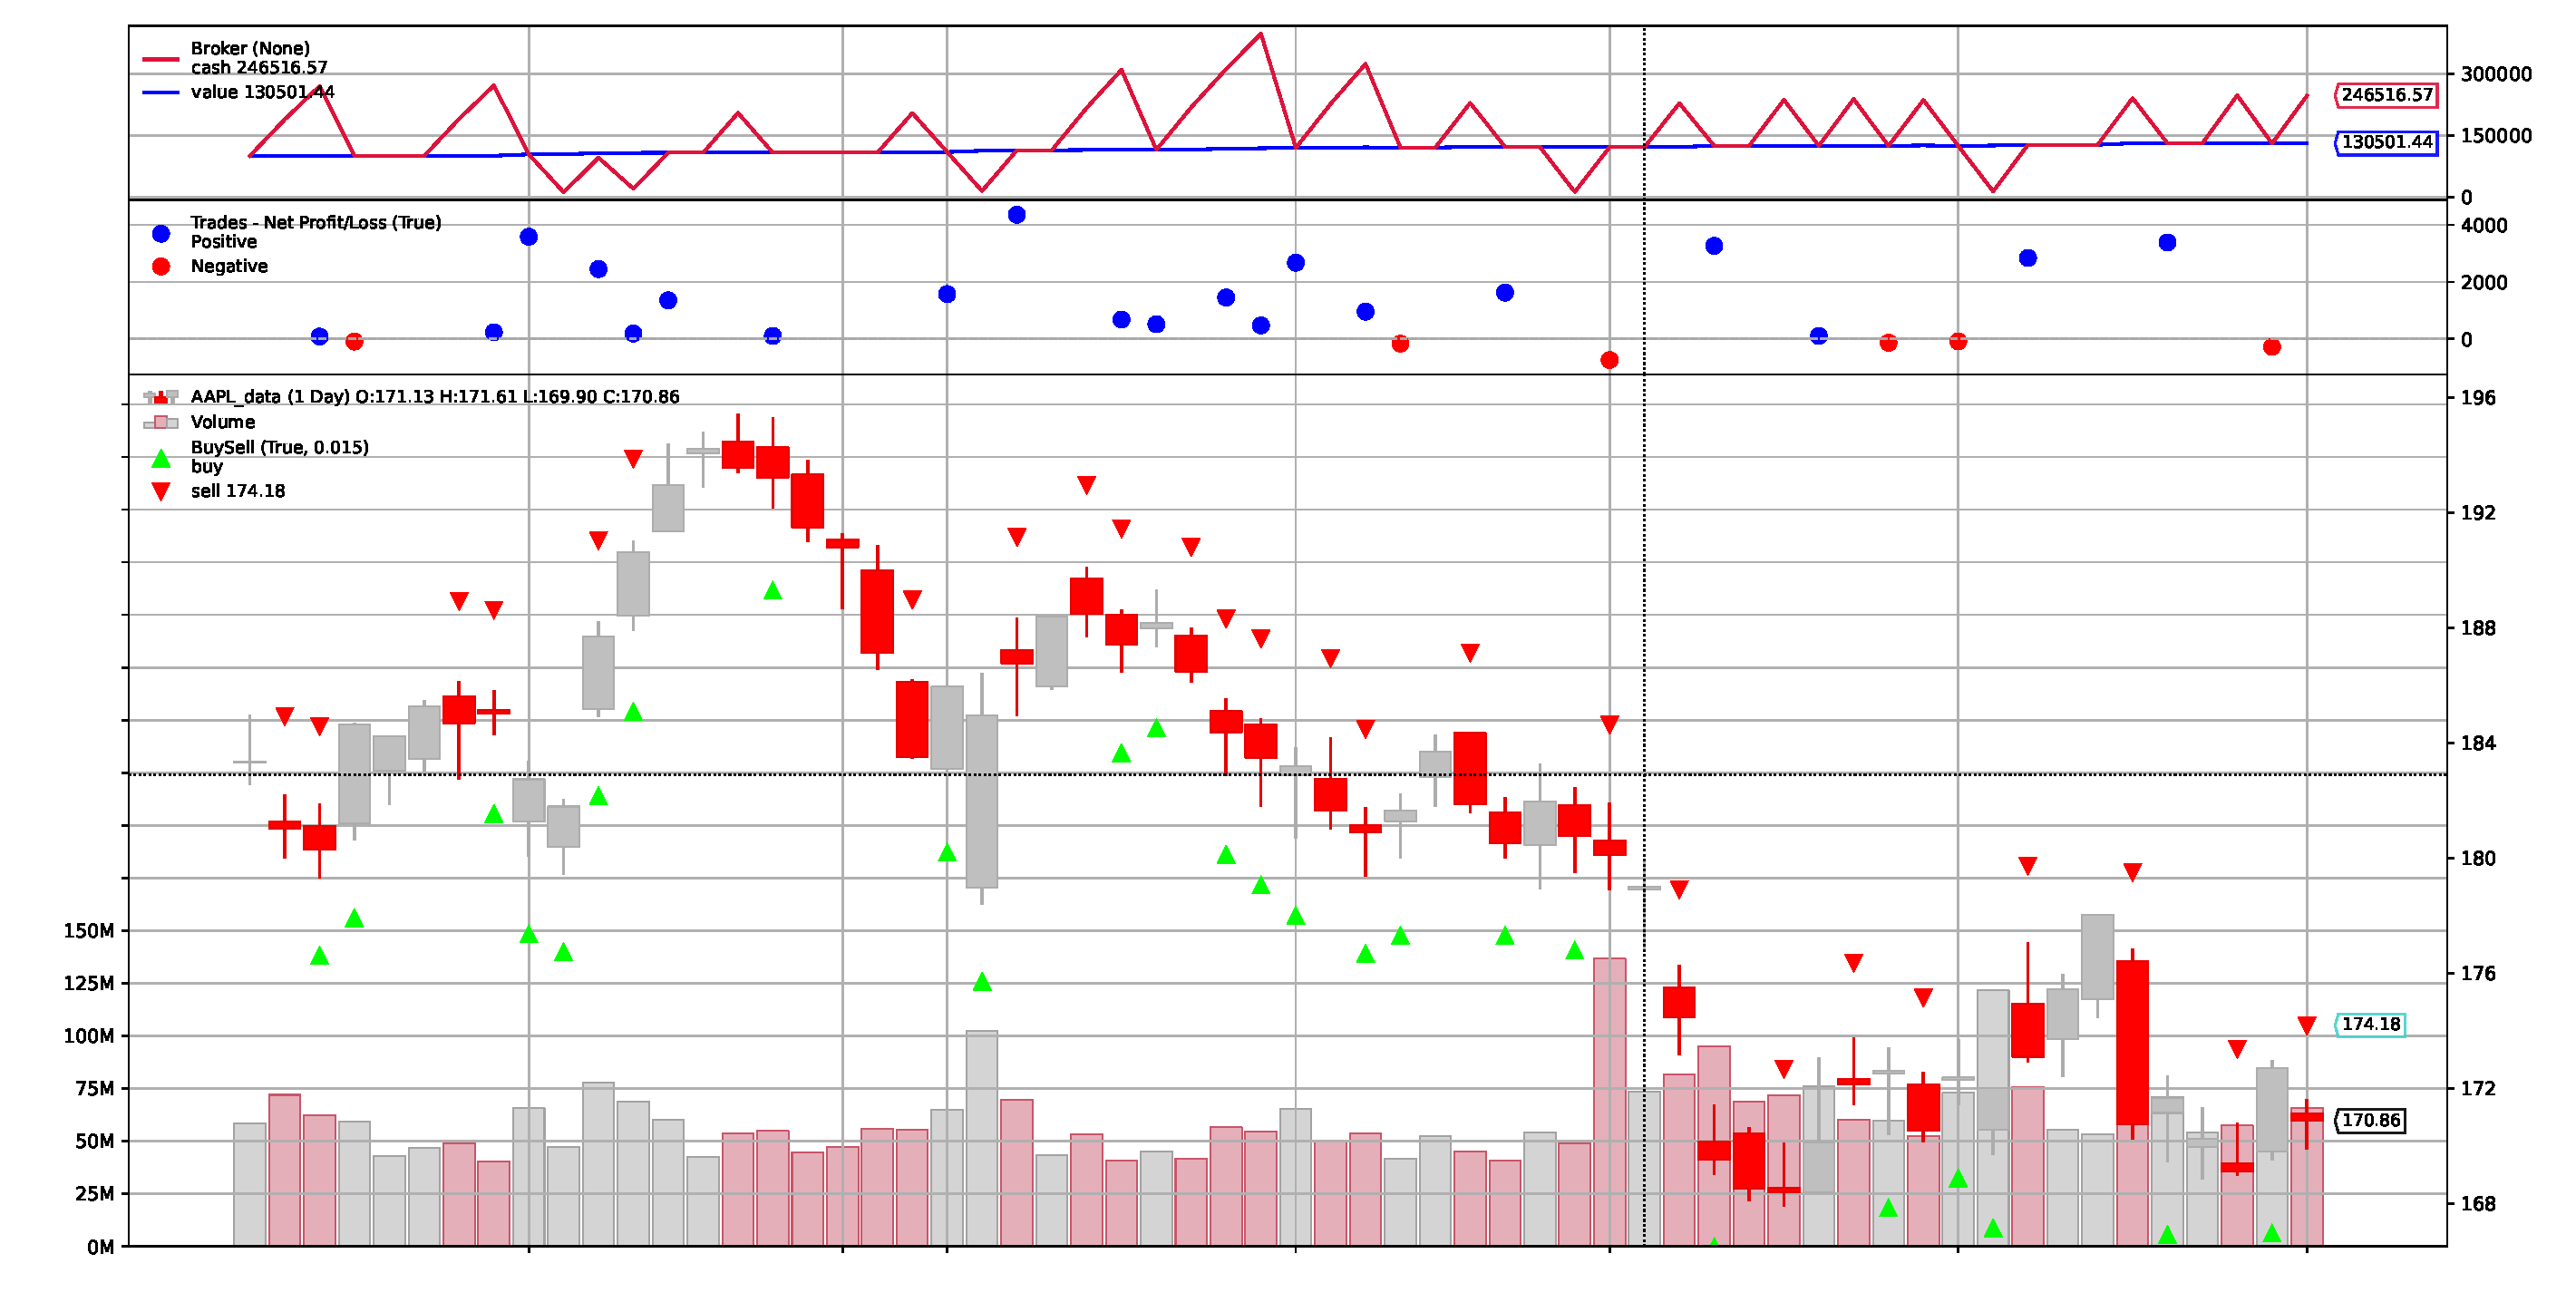
\includegraphics[width=0.95\columnwidth]{figures/AAPL/details.pdf}}
\caption{\textbf{\textcolor{brown}{\model}} Detailed Transaction History for \$AAPL. 
\textcolor{arr_green}{\texttt{Green}} \textcolor{brown}{\textbf{/}} \textcolor{arr_red}{\texttt{Red}} Arrows indicate \textcolor{arr_green}{\texttt{Long}} \textcolor{brown}{\textbf{/}} \textcolor{arr_red}{\texttt{Short}} Positions respectively, showing the model's trading decisions over time.}
\label{fig:aapl-transactions}
\end{center}
\vskip -0.2in
\end{figure}

